\documentclass{scrartcl}

\usepackage[utf8]{inputenc}
\usepackage{amsmath}
\usepackage{csquotes}
\usepackage{tikz}
\usepackage{url}
\usepackage{mdframed}
\usepackage{minted}

\usepackage{hyperref}

\usetikzlibrary{decorations.pathreplacing, angles, quotes, matrix, positioning}

\newcommand{\tushan}{\textsc{Tushan}}

\title{\tushan{}}
\author{Voltidioten}

\begin{document}

\maketitle

This document is the specification of \tushan{}. It contains the 
definitions of game rules, logical entities and their representation and 
protocol specification. The protocol relies on exchanging JSON-messages, hence
every entity of the game is encoded as such.

\section{Game Description}
\tushan{} is based on the game 
\href{https://en.wikipedia.org/wiki/Ta\_Y\%C3\%BC}{Ta-Yü}. Two players
oppose each other on a quadratic field which is separated in cells. Each player 
is assigned two opposite sites of the field. In turns the player place stones
which cover cells. The stones are equipped with connectors on its sites. These
connectors form a flow through the stones. The game ends if there are no valid
placements of the current stone and every player is awarded the product of two
factors, where each factor corresponds to the number of connectors immediately
touching the sites of the field (of said player). These notions are specified
in the following.

\section{Entities}

\subsection{Stone}
\hypertarget{stone}{}
The stones are placed by the players onto the field to form the flow and 
eventually determine the result of the game.

\subsubsection{Description}
A stone is a rectangular shape with a width $n$ and a height $m$. The notions 
of width and height are rastered by the cells, hence any stone covers an 
\hyperlink{area}{\emph{area}} of $n\times m$ cells. The number of connectors is 
variable although throughout one game it usually is consistent. There is at 
least one connector (although for a game with consistent connector numbers 
stones with one connector enforce trivial results). Stones are described in 
terms of $n$ and $m$ and their connectors. Additionally, to incorporate their 
placements in the game we opt to use a representation which contains one 
specific reference cell (the top left corner) and their orientation in terms of 
the direction the top edge is facing (given by one of the four values 
\mintinline{json}{"north"}, \mintinline{json}{"east"}, 
\mintinline{json}{"south"} or \mintinline{json}{"west"}). The connectors are 
identified by indices which move around clockwise (starting by $0$) from the 
top left covered cell.

\subsubsection{Illustration}
\begin{mdframed}
  \begin{center}
    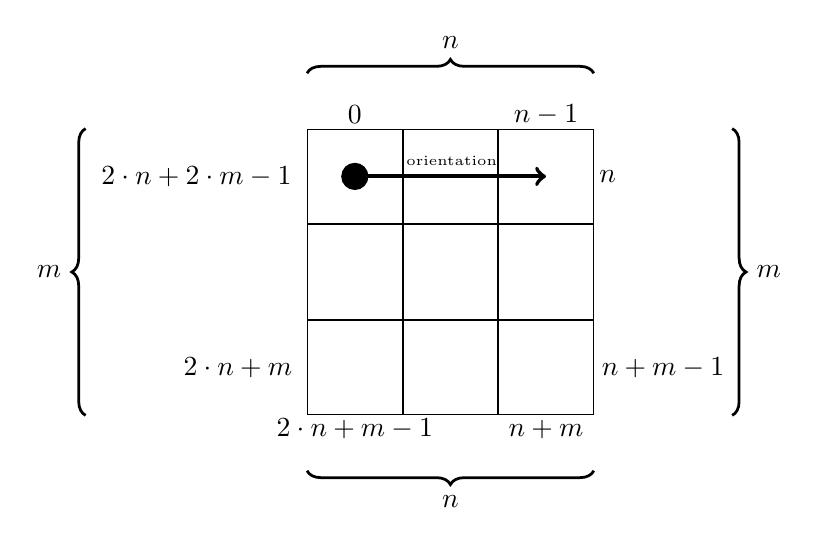
\begin{tikzpicture}
      \matrix (stone) [
        matrix of nodes,
        nodes in empty cells,
        nodes = {
          draw, 
          rectangle,
          anchor = center,
          minimum height = 1.2cm,
          minimum width = 1.2cm,
        }
        ] {
           &  & \\
           &  & \\
           &  & \\
      };
      \draw [ decoration = { brace, amplitude = 5pt, raise = 20pt }, decorate, 
        line width = 1pt ]
          (stone-1-1.north west) -- node [above, yshift = 25pt] {$n$} 
          (stone-1-3.north east);
      \draw [ decoration = { brace, amplitude = 5pt, raise = 80pt }, decorate, 
        line width = 1pt ]
          (stone-3-1.south west) -- node [left, xshift = -85pt] {$m$} 
          (stone-1-1.north west);
      \draw [ decoration = { brace, amplitude = 5pt, raise = 50pt }, decorate, 
        line width = 1pt ]
          (stone-1-3.north east) -- node [right, xshift = 55pt] {$m$} 
          (stone-3-3.south east);
      \draw [ decoration = { brace, amplitude = 5pt, raise = 20pt }, decorate, 
        line width = 1pt ]
          (stone-3-3.south east) -- node [below, yshift = -25pt] {$n$} 
          (stone-3-1.south west);

      \node [yshift = 5pt]   at (stone-1-1.north) {$0$};
      \node [yshift = 5pt]   at (stone-1-3.north) {$n - 1$};
      \node [xshift = 5pt]   at (stone-1-3.east)  {$n$};
      \node [xshift = 25pt]  at (stone-3-3.east)  {$n + m - 1$};
      \node [yshift = -5pt]  at (stone-3-3.south) {$n + m$};
      \node [yshift = -5pt]  at (stone-3-1.south) {$2\cdot n + m - 1$};
      \node [xshift = -25pt] at (stone-3-1.west)  {$2\cdot n + m$};
      \node [xshift = -40pt] at (stone-1-1.west)  {$2\cdot n + 2\cdot m - 1$};

      \node [circle, draw, fill] (orientation start) at (stone-1-1.center) {};
      \draw [->, line width = 1.5pt] (orientation start) to node [above, 
      xshift=-2pt] 
        {\tiny orientation} (stone-1-3.center);
    \end{tikzpicture}
  \end{center}
\end{mdframed}

\subsubsection{Representation}
The encoding of one stone might depend on the fact if it is already placed or 
not. Regardless, we define for any $n,m > 0$ and $c_{0}, \dots, c_{n}$ pairwise
distinct values with $0 \leq c_{i} < 2\cdot n + 2\cdot m$ for $0\leq i\leq n$.
\begin{minted}[escapeinside=||]{text}
  {
    "width": |$n$|,
    "height": |$m$|,
    "connectors": [|$c_0, \dots, c_n$|]
  }
\end{minted}
If the stone is placed in a \hyperlink{field}{\emph{field}} this is indicated 
by the inclusion of an additional object with key 
\mintinline{json}{"position"}. Here valid ranges of coordinates $x, y \geq 0$ 
depend on the \hyperlink{field}{\emph{field}} the stone is placed in while $o$ 
is always one of the values \mintinline{json}{"north"}, 
\mintinline{json}{"east"}, \mintinline{json}{"south"} or 
\mintinline{json}{"west"}.
\begin{minted}[escapeinside=||]{text}
  {
    "width": |$n$|,
    "height": |$m$|,
    "connectors": [|$c_0, \dots, c_n$|],
    "position": {
      "x": |$x$|,
      "y": |$y$|,
      "orientation": |$o$|
    }
  }
\end{minted}

\subsubsection{Associated Notions}
\begin{mdframed}
  \hypertarget{area}{\emph{Area of placed stone}} - The area of a placed stone 
  is defined by all cells it covers, namely all cells with coordinates 
  \begin{equation*}
    (a, b) \text{ s. t. }
    \begin{cases}
      x\leq b\leq x + m - 1, y - n + 1\leq a\leq y &\text{if }o = \texttt{"north"}\\
      x\leq a\leq x + n - 1, y\leq b\leq y + m - 1 &\text{if }o = \texttt{"east"}\\
      x - m + 1\leq b\leq x, y\leq a\leq y + n - 1 &\text{if }o = \texttt{"south"}\\
      x - n + 1\leq a\leq x, y - m + 1\leq b\leq y &\text{if }o = \texttt{"west"}\\
    \end{cases}
  \end{equation*}
  where $o$ is the orientation of the stone and $x, y$ its respective $x$- and
  $y$-coordinate.
\end{mdframed}
\begin{mdframed}
  \hypertarget{initial}{\emph{Initial stone}} - A stone is called initial if it 
  is the only stone placed onto a \hyperlink{field}{\emph{field}}. The 
  \hyperlink{area}{\emph{area}} of any initial stone must contain one of the 
  following cells
  \begin{itemize}
    \item $(\frac{n}{2}, \frac{n}{2})$,
    \item $(\frac{n}{2} + 1, \frac{n}{2})$,
    \item $(\frac{n}{2}, \frac{n}{2} + 1)$,
    \item $(\frac{n}{2} + 1, \frac{n}{2} + 1)$.
  \end{itemize}
\end{mdframed}
\begin{mdframed}
  \hypertarget{valid}{\emph{Validity of placed stones}} - A stone is considered 
  validly placed if its \hyperlink{area}{\emph{area}} is inside the field; that 
  is if for all $(a, b)$ in its area $1\leq a, b\leq d$ for a 
  \hyperlink{field}{\emph{field}} with dimension $d$. Furthermore, it holds 
  that \emph{every} connector is connected either to one of the delimiting 
  walls, to another connector or an empty cell. Additionally, the stone is 
  either \hyperlink{initial}{\emph{initial}} or there is at least \emph{one} 
  connector that is adjacent to another connector.
\end{mdframed}

\subsubsection{Example}
We consider the following stone and its encoding
\begin{mdframed}
  \begin{minipage}{0.5\textwidth}
    \inputminted{json}{examples/not-placed-stone.json}
  \end{minipage}%
  \begin{minipage}{0.5\textwidth}
    \begin{center}
      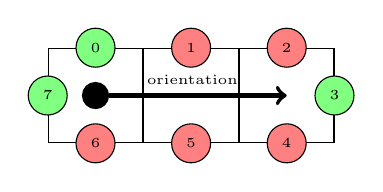
\begin{tikzpicture}
        \matrix (stone) [
          matrix of nodes,
          nodes in empty cells,
          nodes = {
            draw, 
            rectangle,
            anchor = center,
            minimum height = 1.2cm,
            minimum width = 1.2cm,
          }
        ] {
           &  & \\
        };
        \node [fill = green!50, circle, draw] (c0) at (stone-1-1.north) {
          \tiny{0}};
        \node [fill = red!50, circle, draw]   (c1) at (stone-1-2.north) {
          \tiny{1}};
        \node [fill = red!50, circle, draw]   (c2) at (stone-1-3.north) {
          \tiny{2}};
        \node [fill = green!50, circle, draw] (c3) at (stone-1-3.east)  {
          \tiny{3}};
        \node [fill = red!50, circle, draw]   (c4) at (stone-1-3.south) {
          \tiny{4}};
        \node [fill = red!50, circle, draw]   (c5) at (stone-1-2.south) {
          \tiny{5}};
        \node [fill = red!50, circle, draw]   (c6) at (stone-1-1.south) {
          \tiny{6}};
        \node [fill = green!50, circle, draw] (c7) at (stone-1-1.west)  {
          \tiny{7}};

        \node [circle, draw, fill] (orientation start) at (stone-1-1.center) {};
        \draw [->, line width = 1.5pt] (orientation start) to node [above, 
        xshift=-2pt] 
          {\tiny orientation} (stone-1-3.center);
      \end{tikzpicture}
    \end{center}
    \tiny{Green circles indicate a connector while red circles mark positions of
    possible but for this stone not available connectors.}
 \end{minipage}%
\end{mdframed}

Additionally, we might encounter this stone after its already placed, e.g.
\begin{mdframed}
  \begin{minipage}{0.5\textwidth}
    \inputminted{json}{examples/placed-stone.json}
  \end{minipage}%
  \begin{minipage}{0.5\textwidth}
    \begin{center}
      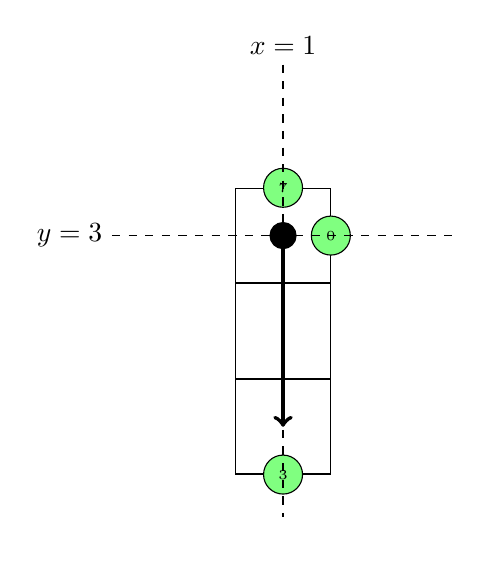
\begin{tikzpicture}
        \matrix (stone) [
          matrix of nodes,
          nodes in empty cells,
          nodes = {
            draw, 
            rectangle,
            anchor = center,
            minimum height = 1.2cm,
            minimum width = 1.2cm,
          }
        ] {
           \\
           \\
           \\
        };
        \node [fill = green!50, circle, draw] (c0) at (stone-1-1.east)  {
          \tiny{0}};
        \node [fill = green!50, circle, draw] (c0) at (stone-3-1.south) {
          \tiny{3}};
        \node [fill = green!50, circle, draw] (c0) at (stone-1-1.north) {
          \tiny{7}};

        \node [circle, draw, fill] (orientation start) at (stone-1-1.center) {};
        \draw [->, line width = 1.5pt] (orientation start) to (stone-3-1.center);

        \node [left  = 2 of orientation start] (ystart) {$y = 3$};
        \node [right = 2 of orientation start] (yend)   {};

        \node [above = 2 of orientation start] (xstart) {$x = 1$};
        \node [below = 3.4 of orientation start] (xend)   {};

        \draw [dashed] (ystart) to (yend);
        \draw [dashed] (xstart) to (xend);
      \end{tikzpicture}
    \end{center}
  \end{minipage}%
\end{mdframed}


\subsection{Field}
\hypertarget{field}{}
The field of the game.

\subsubsection{Description}
The field is a quadratic collection of cells. Each cell is identified by its 
coordinates starting with $(0,0)$ at the top left and proceeding to the left 
with increasing first element and to the bottom with increasing second element,
this corresponds to a discrete cartesian coordinate system starting at the top
left growing right- and downwards. The four values \enquote{north}, 
\enquote{east}, \enquote{south} and \enquote{west} refer to the top, left, 
bottom and right side respectively and are especially relevant for the 
orientation of placed \hyperlink{stone}{\emph{stones}}.

\subsubsection{Illustration}
\begin{mdframed}
  \begin{center}
    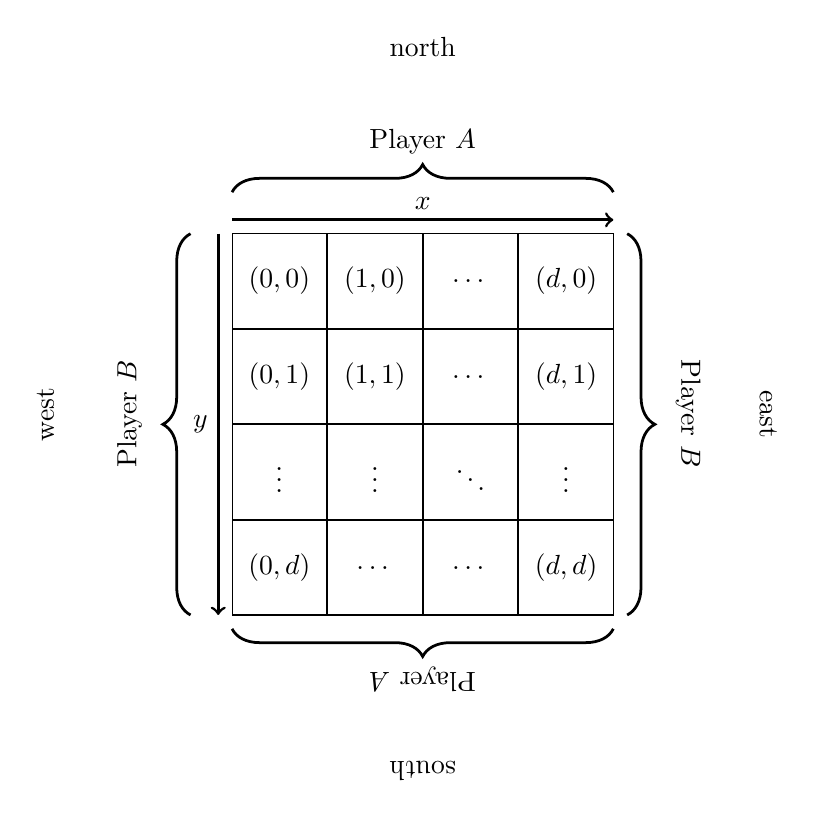
\begin{tikzpicture}
      \matrix (field) [
        matrix of nodes,
        column sep = 0pt,
        row sep = 0pt,
        nodes in empty cells,
        inner xsep = 0pt,
        nodes = {
          rectangle, draw, minimum width = 1.2cm, minimum height = 1.2cm, 
          outer sep = 0pt, inner xsep = 0pt, inner ysep = 0pt, anchor = center
        }] {
          $(0,0) $ & $(1,0) $ & $\dots $ & $(d,0) $ \\
          $(0,1) $ & $(1,1) $ & $\dots $ & $(d,1) $ \\
          $\vdots$ & $\vdots$ & $\ddots$ & $\vdots$ \\
          $(0,d) $ & $\dots $ & $\dots $ & $(d,d) $ \\
      };
      \draw [ decoration = { brace, raise = 15pt, amplitude = 10pt }, decorate, 
        line width = 1pt ]
          (field-1-1.north west) -- node [above, yshift = 25pt] {Player $A$} 
          (field-1-4.north east);
      \draw [ decoration = { brace, raise = 5pt, amplitude = 10pt, mirror }, 
        decorate, line width = 1pt ]
          (field-4-1.south west) -- node [below, yshift = -15pt, label = {
            [rotate = 180] {Player $A$}}] {} (field-4-4.south east);
      \draw [ draw, -> , line width = 1pt] ([yshift = 5pt] field-1-1.north west) 
        to node [above] {$x$} ([yshift = 5pt] field-1-4.north east);
      \draw [ draw, -> , line width = 1pt] ([xshift = -5pt] field-1-1.north west) 
        to node [left] {$y$} ([xshift = -5pt] field-4-1.south west);
      \draw [ decoration = { brace, raise = 15pt, amplitude = 10pt, mirror }, 
        decorate, line width = 1pt ]
          (field-1-1.north west) -- node [left, xshift = -25pt, label = {
            [rotate = 90] {Player $B$}}] {} (field-4-1.south west);
      \draw [ decoration = { brace, raise = 5pt, amplitude = 10pt }, 
        decorate, line width = 1pt ]
          (field-1-4.north east) -- node [right, xshift = 15pt, label = {
            [rotate = -90] {Player $B$}}] {} 
          (field-4-4.south east);

      \node [above = 2 of field] (n) {north};
      \node [right = 1.6 of field, label = {[rotate = -90] {east}}] {};
      \node [below = 1.6 of field, label = {[rotate = 180] {south}}] {};
      \node [left  = 2 of field, label = {[rotate = 90] {west}}] {};
    \end{tikzpicture}
  \end{center}
\end{mdframed}

\subsubsection{Representation}
The parameter of a field are its dimension $d$ and placed 
\hyperlink{stone}{\emph{stones}}. Therefore, we define for $d > 1$ and
\hyperlink{valid}{\emph{validly placed}} \hyperlink{stone}{\emph{stones}}
$s_{1}, \dots, s_{k}$ its representation as
\begin{minted}[escapeinside=||]{text}
  {
    "dimension": |$d$|,
    "stones": [|$s_1, \dots, s_k$|]
  }
\end{minted}

\end{document}
